\section{问题重述与总体分析}
\subsection{场景与研究任务}
本文以赛题给定的镇龙乡及周边山区标准场景为研究对象\textsuperscript{\cite{D2026}}。调度中心O01负责向15个服务区配送80个不可拆货箱，物资包括饮用水、应急食品、医疗物资和生活卫生用品。可用运输装备由三种机型、八架实体无人机和配套共享电池组成；在固定网关不能提供直接通信的区域，还可调用中继无人机与可更换能源组件。

运输方案的可执行性由空间、时间和资源共同决定。空间上，航段须保持沿线地形净空，山地爬升会改变能耗；时间上，医疗箱和首批保障箱受硬截止约束，其他货箱存在及时性要求；资源上，同一架无人机不能同时执行多个任务，电池返航后也不能立即视为满电。通信进一步把运输轨迹和中继在位时段联系起来：一条路线即使能量可行，也可能因某段飞行缺少可用链路而不可执行。

\subsection{四个问题的层次与衔接}
问题一在单服务区直接往返条件下研究运输能力和组批。每个服务区单独处理，既不跨服务区拼箱，也不安排具体实体机和电池。其作用是建立一致的航段计算规则，得到单点任务的容量边界和可行批次。

问题二允许同一架次访问多个服务区，联合确定组批、访问顺序、机型、实体机、电池与开始时刻。多点串访可减少重复往返，但增加后续货箱的等待，并改变各航段的剩余载荷。因此，不能只比较总里程，也不能把问题一的架次直接并行排列后视为调度完成。

问题三把连续通信加入问题二。中继任务需提前飞抵并完成建链，服务结束后还要返航，其在位时长同时受到能源和设备周转限制。运输开始时刻变化会移动通信需求区间；中继不可及时就位时，则需要调整运输时序或任务组织。

问题四以有效的问题三联合方案为固定输入，分别划分两个和三个独立任务组。此时研究重点从重新优化路线转向固定任务的归属与资源核算。同架次共访的服务区必须同组，跨组资源不得调配，通信保障关系也不能随分组任意改写。

上述依赖关系见图\ref{fig:overall}。四问共用节点编号、物理参数、能耗与时间口径；后一问增加约束或改变执行组织形式，但不另设一套基础计算规则。
\begin{figure}[H]\centering
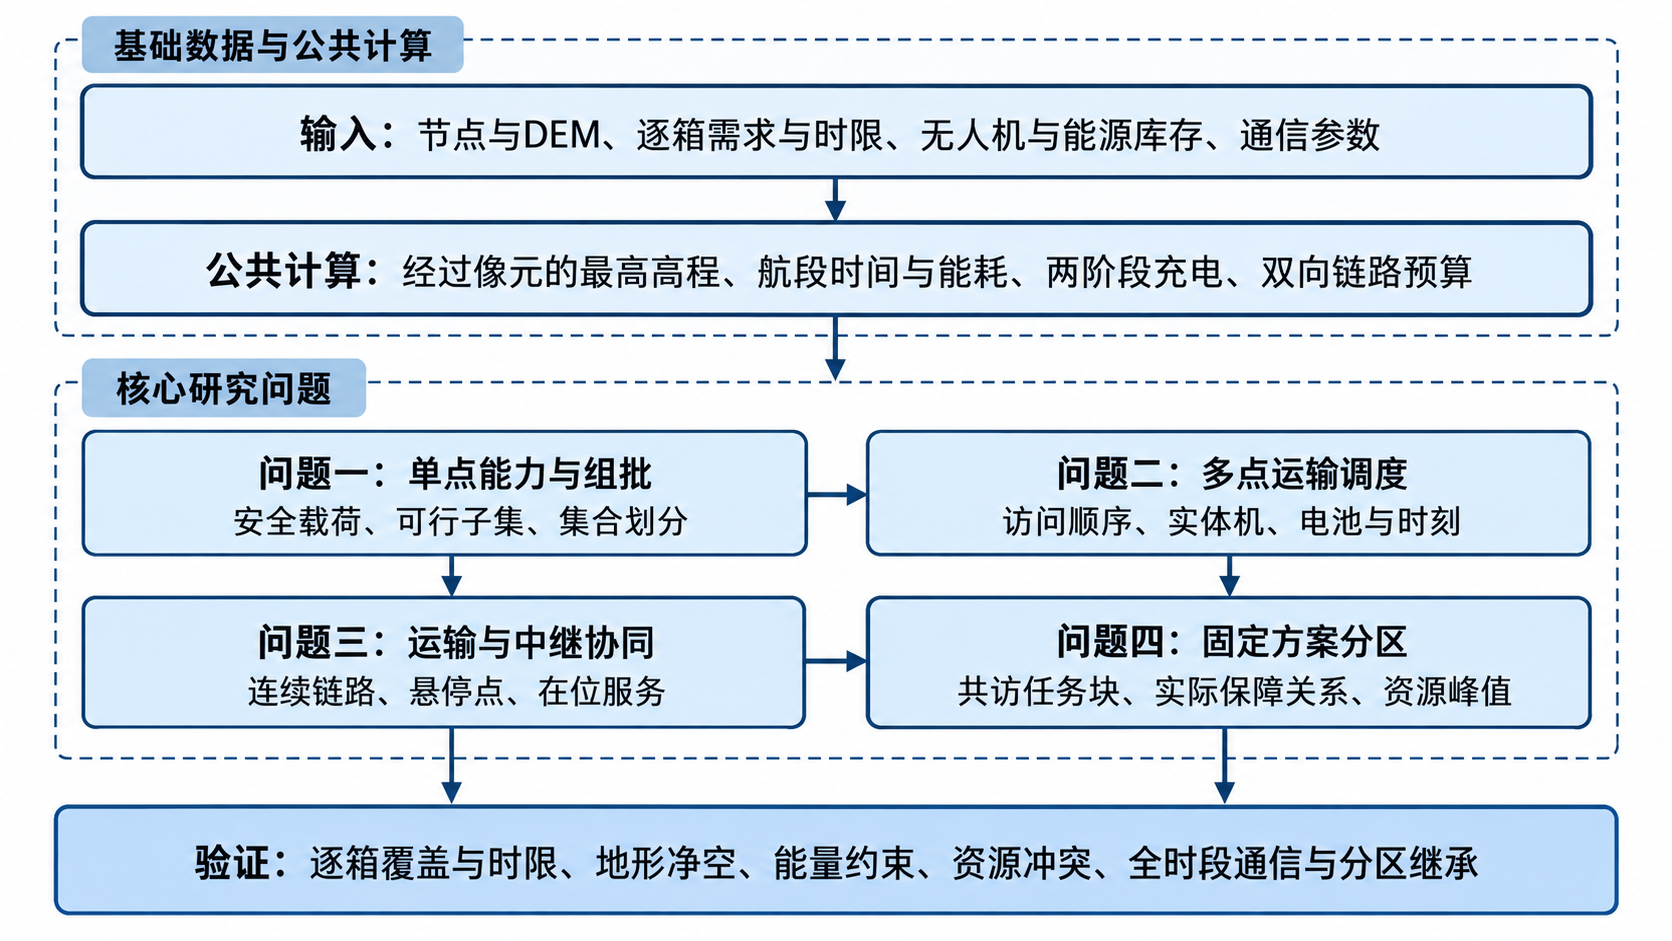
\includegraphics[width=.86\textwidth]{figures/common/figure1.png}
\caption{四个子问题的输入、方法与输出依赖关系}\label{fig:overall}
\end{figure}

\subsection{研究策略与评价原则}
本文采用可行性优先的建模策略。载质量、装载体积、返航电量、硬截止以及资源占用构成不可违反的约束；在可行集合内，再比较迟到、完工时间、能耗和架次数。这样可以避免通过降低安全余量或容忍医疗箱逾期，换取表面上的目标改善。

不同层次的最优性应分别表述。单点组批可在完整候选集合上进行精确动态规划；多点运输与中继联合调度采用构造与事件仿真方法时，只能说明所获候选方案的表现。固定时序下的任务分区若穷尽全部合法划分，可讨论该固定方案及所选评价口径下的最优分区，不能据此推及整体运输通信问题的全局最优。
